%-----------------------------------------------------------------------------------------
% Autor dieser Vorlage:
% Stefan Macke (http://fachinformatiker-anwendungsentwicklung.net)
% Permalink zur Vorlage: http://fiae.link/LaTeXVorlageFIAE
%
% Sämtliche verwendeten Abbildungen, Tabellen und Listings stammen von Dirk Grashorn.
%
% Lizenz: Creative Commons 4.0 Namensnennung - Weitergabe unter gleichen Bedingungen
% -----------------------------------------------------------------------------------------

\documentclass[
	ngerman,
	toc=listof, % Abbildungsverzeichnis sowie Tabellenverzeichnis in das Inhaltsverzeichnis aufnehmen
	toc=bibliography, % Literaturverzeichnis in das Inhaltsverzeichnis aufnehmen
	footnotes=multiple, % Trennen von direkt aufeinander folgenden Fußnoten
	parskip=half, % vertikalen Abstand zwischen Absätzen verwenden anstatt horizontale Einrückung von Folgeabsätzen
	numbers=noendperiod % Den letzten Punkt nach einer Nummerierung entfernen (nach DIN 5008)
]{scrartcl}
\pdfminorversion=5 % erlaubt das Einfügen von pdf-Dateien bis Version 1.7, ohne eine Fehlermeldung zu werfen (keine Garantie für fehlerfreies Einbetten!)
\usepackage[utf8]{inputenc} % muss als erstes eingebunden werden, da Meta/Packages ggfs. Sonderzeichen enthalten

% !TEX root = Projektdokumentation.tex

% Hinweis: der Titel muss zum Inhalt des Projekts passen und den zentralen Inhalt des Projekts deutlich herausstellen
\newcommand{\titel}{Automatisierte Onboarding Prozesse}
\newcommand{\untertitel}{Implementierung automatisierter
Onboarding- und Ressourcenmanagement-Prozesse zur Optimierung der User Experience für neue
Entwickler bei TUI Group}
\newcommand{\kompletterTitel}{\titel{} -- \untertitel}

\newcommand{\autorName}{Paul Glesmann}
\newcommand{\autorAnschrift}{Schopenhauerstraße 15}
\newcommand{\autorOrt}{30625 Hannover}

\newcommand{\betriebLogo}{tuilogo.png}
\newcommand{\betriebName}{\textsc{} TUI InfoTec GmbH}
\newcommand{\betriebAnschrift}{Karl-Wiechert-Allee 23}
\newcommand{\betriebOrt}{30625 Hannover}

\newcommand{\ausbildungsberuf}{Fachinformatiker für Anwendungsentwicklung}
\newcommand{\betreff}{Dokumentation zur betrieblichen Projektarbeit}
\newcommand{\pruefungstermin}{Winter 2024}
\newcommand{\abgabeOrt}{Hannover}
\newcommand{\abgabeTermin}{18.11.2024}
 % Metadaten zu diesem Dokument (Autor usw.)
% !TEX root = ../Projektdokumentation.tex

% Anpassung an Landessprache ---------------------------------------------------
\usepackage{babel}

% Umlaute ----------------------------------------------------------------------
%   Umlaute/Sonderzeichen wie äüöß direkt im Quelltext verwenden (CodePage).
%   Erlaubt automatische Trennung von Worten mit Umlauten.
% ------------------------------------------------------------------------------
\usepackage[T1]{fontenc}
\usepackage{textcomp} % Euro-Zeichen etc.

% Schrift ----------------------------------------------------------------------
\usepackage{lmodern} % bessere Fonts
\usepackage{relsize} % Schriftgröße relativ festlegen

% Tabellen ---------------------------------------------------------------------
\PassOptionsToPackage{table}{xcolor}
\usepackage{tabularx}
% für lange Tabellen
\usepackage{longtable}
\usepackage{array}
\usepackage{ragged2e}
\usepackage{lscape}
\newcolumntype{w}[1]{>{\raggedleft\hspace{0pt}}p{#1}} % Spaltendefinition rechtsbündig mit definierter Breite

% Grafiken ---------------------------------------------------------------------
\usepackage[dvips,final]{graphicx} % Einbinden von JPG-Grafiken ermöglichen
\usepackage{graphics} % keepaspectratio
\usepackage{floatflt} % zum Umfließen von Bildern
\graphicspath{{Bilder/}} % hier liegen die Bilder des Dokuments

% Sonstiges --------------------------------------------------------------------
\usepackage[titles]{tocloft} % Inhaltsverzeichnis DIN 5008 gerecht einrücken
\usepackage{amsmath,amsfonts} % Befehle aus AMSTeX für mathematische Symbole
\usepackage{enumitem} % anpassbare Enumerates/Itemizes
\usepackage{xspace} % sorgt dafür, dass Leerzeichen hinter parameterlosen Makros nicht als Makroendezeichen interpretiert werden

\usepackage{makeidx} % für Index-Ausgabe mit \printindex
\usepackage[printonlyused]{acronym} % es werden nur benutzte Definitionen aufgelistet

% Einfache Definition der Zeilenabstände und Seitenränder etc.
\usepackage{setspace}
\usepackage{geometry}

% Symbolverzeichnis
\usepackage[intoc]{nomencl}
\let\abbrev\nomenclature
\renewcommand{\nomname}{Abkürzungsverzeichnis}
\setlength{\nomlabelwidth}{.25\hsize}
\renewcommand{\nomlabel}[1]{#1 \dotfill}
\setlength{\nomitemsep}{-\parsep}

\usepackage{varioref} % Elegantere Verweise. „auf der nächsten Seite“
\usepackage{url} % URL verlinken, lange URLs umbrechen etc.

\usepackage{chngcntr} % fortlaufendes Durchnummerieren der Fußnoten
% \usepackage[perpage]{footmisc} % Alternative: Nummerierung der Fußnoten auf jeder Seite neu

\usepackage{ifthen} % bei der Definition eigener Befehle benötigt
\usepackage{todonotes} % definiert u.a. die Befehle \todo und \listoftodos
\usepackage[square]{natbib} % wichtig für korrekte Zitierweise

% PDF-Optionen -----------------------------------------------------------------
\usepackage{pdfpages}
\pdfminorversion=5 % erlaubt das Einfügen von pdf-Dateien bis Version 1.7, ohne eine Fehlermeldung zu werfen (keine Garantie für fehlerfreies Einbetten!)
\usepackage[
    bookmarks,
    bookmarksnumbered,
    bookmarksopen=true,
    bookmarksopenlevel=1,
    colorlinks=true,
% diese Farbdefinitionen zeichnen Links im PDF farblich aus
    anchorcolor=AOBlau,% Ankertext
    citecolor=AOBlau, % Verweise auf Literaturverzeichniseinträge im Text
    filecolor=AOBlau, % Verknüpfungen, die lokale Dateien öffnen
    menucolor=AOBlau, % Acrobat-Menüpunkte
    urlcolor=AOBlau,
% diese Farbdefinitionen sollten für den Druck verwendet werden (alles schwarz)
    %linkcolor=black, % einfache interne Verknüpfungen
    %anchorcolor=black, % Ankertext
    %citecolor=black, % Verweise auf Literaturverzeichniseinträge im Text
    %filecolor=black, % Verknüpfungen, die lokale Dateien öffnen
    %menucolor=black, % Acrobat-Menüpunkte
    %urlcolor=black,
%
    %backref, % Quellen werden zurück auf ihre Zitate verlinkt
    pdftex,
    plainpages=false, % zur korrekten Erstellung der Bookmarks
    pdfpagelabels=true, % zur korrekten Erstellung der Bookmarks
    hypertexnames=false, % zur korrekten Erstellung der Bookmarks
    linkcolor=AOBlau,
    linktoc=page
]{hyperref}
% Befehle, die Umlaute ausgeben, führen zu Fehlern, wenn sie hyperref als Optionen übergeben werden
\hypersetup{
    pdftitle={\titel -- \untertitel},
    pdfauthor={\autorName},
    pdfcreator={\autorName},
    pdfsubject={\titel -- \untertitel},
    pdfkeywords={\titel -- \untertitel},
}

% zum Einbinden von Programmcode -----------------------------------------------
\usepackage{listings}
\usepackage{xcolor}
\definecolor{hellgelb}{rgb}{1,1,0.9}
\definecolor{colKeys}{rgb}{0,0,1}
\definecolor{colIdentifier}{rgb}{0,0,0}
\definecolor{colComments}{rgb}{0,0.5,0}
\definecolor{colString}{rgb}{1,0,0}
\usepackage[acronym]{glossaries}

\lstset{
    float=hbp,
	basicstyle=\footnotesize,
    identifierstyle=\color{colIdentifier},
    keywordstyle=\color{colKeys},
    stringstyle=\color{colString},
    commentstyle=\color{colComments},
    backgroundcolor=\color{hellgelb},
    columns=flexible,
    tabsize=2,
    frame=single,
    extendedchars=true,
    showspaces=false,
    showstringspaces=false,
    numbers=left,
    numberstyle=\tiny,
    breaklines=true,
    breakautoindent=true,
	captionpos=b,
}
\lstdefinelanguage{cs}{
	sensitive=false,
	morecomment=[l]{//},
	morecomment=[s]{/*}{*/},
	morestring=[b]",
	morekeywords={
		abstract,event,new,struct,as,explicit,null,switch
		base,extern,object,this,bool,false,operator,throw,
		break,finally,out,true,byte,fixed,override,try,
		case,float,params,typeof,catch,for,private,uint,
		char,foreach,protected,ulong,checked,goto,public,unchecked,
		class,if,readonly,unsafe,const,implicit,ref,ushort,
		continue,in,return,using,decimal,int,sbyte,virtual,
		default,interface,sealed,volatile,delegate,internal,short,void,
		do,is,sizeof,while,double,lock,stackalloc,
		else,long,static,enum,namespace,string},
}
\lstdefinelanguage{natural}{
	sensitive=false,
	morecomment=[l]{/*},
	morestring=[b]",
	morestring=[b]',
	alsodigit={-,*},
	morekeywords={
		DEFINE,DATA,LOCAL,END-DEFINE,WRITE,CALLNAT,PARAMETER,USING,
		IF,NOT,END-IF,ON,*ERROR-NR,ERROR,END-ERROR,ESCAPE,ROUTINE,
		PERFORM,SUBROUTINE,END-SUBROUTINE,CONST,END-FOR,END,FOR,RESIZE,
		ARRAY,TO,BY,VALUE,RESET,COMPRESS,INTO,EQ},
}
\lstdefinelanguage{php}{
	sensitive=false,
	morecomment=[l]{/*},
	morestring=[b]",
	morestring=[b]',
	alsodigit={-,*},
	morekeywords={
		abstract,and,array,as,break,case,catch,cfunction,class,clone,const,
		continue,declare,default,do,else,elseif,enddeclare,endfor,endforeach,
		endif,endswitch,endwhile,extends,final,for,foreach,function,global,
		goto,if,implements,interface,instanceof,namespace,new,old_function,or,
		private,protected,public,static,switch,throw,try,use,var,while,xor
		die,echo,empty,exit,eval,include,include_once,isset,list,require,
		require_once,return,print,unset},
}
 % verwendete Packages
% !TEX root = ../Projektdokumentation.tex

% Seitenränder -----------------------------------------------------------------
\setlength{\topskip}{\ht\strutbox} % behebt Warnung von geometry
\geometry{a4paper,left=20mm,right=20mm,top=25mm,bottom=35mm}

\usepackage[
	automark, % Kapitelangaben in Kopfzeile automatisch erstellen
	headsepline, % Trennlinie unter Kopfzeile
	ilines % Trennlinie linksbündig ausrichten
]{scrlayer-scrpage}

% Kopf- und Fußzeilen ----------------------------------------------------------
\pagestyle{scrheadings}
% chapterpagestyle gibt es nicht in scrartcl
%\renewcommand{\chapterpagestyle}{scrheadings}
\clearscrheadfoot

% Kopfzeile
\renewcommand{\headfont}{\normalfont} % Schriftform der Kopfzeile
\ihead{\large{\textsc{\titel}}\\ \small{Implementierung automatisierter Onboarding- und Ressourcenmanagement-Prozesse \newline zur Optimierung der
User Experience für neue Entwickler bei TUI Group} \\[2ex] \textit{\headmark}}
\chead{}
\ohead{\includegraphics[scale=0.2]{\betriebLogo}}
\setlength{\headheight}{15mm} % Höhe der Kopfzeile
%\setheadwidth[0pt]{textwithmarginpar} % Kopfzeile über den Text hinaus verbreitern (falls Logo den Text überdeckt)

% Fußzeile
\ifoot{\autorName}
\cfoot{}
\ofoot{\pagemark}

% Überschriften nach DIN 5008 in einer Fluchtlinie
% ------------------------------------------------------------------------------

% Abstand zwischen Nummerierung und Überschrift definieren
% > Schön wäre hier die dynamische Berechnung des Abstandes in Abhängigkeit
% > der Verschachtelungstiefe des Inhaltsverzeichnisses
\newcommand{\headingSpace}{1.5cm}

% Abschnittsüberschriften im selben Stil wie beim Inhaltsverzeichnis einrücken
\renewcommand*{\othersectionlevelsformat}[3]{
  \makebox[\headingSpace][l]{#3\autodot}
}

% Für die Einrückung wird das Paket tocloft benötigt
%\cftsetindents{chapter}{0.0cm}{\headingSpace}
\cftsetindents{section}{0.0cm}{\headingSpace}
\cftsetindents{subsection}{0.0cm}{\headingSpace}
\cftsetindents{subsubsection}{0.0cm}{\headingSpace}
\cftsetindents{figure}{0.0cm}{\headingSpace}
\cftsetindents{table}{0.0cm}{\headingSpace}


% Allgemeines
% ------------------------------------------------------------------------------

\onehalfspacing % Zeilenabstand 1,5 Zeilen
\frenchspacing % erzeugt ein wenig mehr Platz hinter einem Punkt

% Schusterjungen und Hurenkinder vermeiden
\clubpenalty = 10000
\widowpenalty = 10000
\displaywidowpenalty = 10000

% Quellcode-Ausgabe formatieren
\lstset{numbers=left, numberstyle=\tiny, numbersep=5pt, breaklines=true}
\lstset{emph={square}, emphstyle=\color{red}, emph={[2]root,base}, emphstyle={[2]\color{blue}}}

\counterwithout{footnote}{section} % Fußnoten fortlaufend durchnummerieren
\setcounter{tocdepth}{3} % im Inhaltsverzeichnis werden die Kapitel bis zum Level der subsubsection übernommen
\setcounter{secnumdepth}{3} % Kapitel bis zum Level der subsubsection werden nummeriert

% Aufzählungen anpassen
\renewcommand{\labelenumi}{\arabic{enumi}.}
\renewcommand{\labelenumii}{\arabic{enumi}.\arabic{enumii}.}
\renewcommand{\labelenumiii}{\arabic{enumi}.\arabic{enumii}.\arabic{enumiii}}

% Tabellenfärbung:
\definecolor{heading}{rgb}{0.64,0.78,0.86}
\definecolor{odd}{rgb}{0.9,0.9,0.9}
 % Definitionen zum Aussehen der Seiten
\input{Allgemein/Befehle} % eigene allgemeine Befehle, die z.B. die Arbeit mit LaTeX erleichtern
\input{Befehle} % eigene projektspezifische Befehle, z.B. Abkürzungen usw.

\begin{document}

% \phantomsection
% \thispagestyle{empty}
% \pdfbookmark[1]{Eidesstattliche Erklärung}{ihkdeckblatt}
% \includegraphicsKeepAspectRatio{DeckblattIHK}{1}
% \cleardoublepage

\phantomsection
\thispagestyle{plain}
\pdfbookmark[1]{Deckblatt}{deckblatt}
\input{Deckblatt}
\cleardoublepage

% Preface --------------------------------------------------------------------
\phantomsection
\pagenumbering{Roman}
\pdfbookmark[1]{Inhaltsverzeichnis}{inhalt}
\tableofcontents

\cleardoublepage

\phantomsection
\listoffigures
\cleardoublepage

\phantomsection
\listoftables
\cleardoublepage

\phantomsection
\lstlistoflistings
\cleardoublepage

\newcommand{\abkvz}{Abkürzungsverzeichnis}
\renewcommand{\nomname}{\abkvz}
\section*{\abkvz}
\markboth{\abkvz}{\abkvz}
\addcontentsline{toc}{section}{\abkvz}
% !TEX root = Projektdokumentation.tex

% Es werden nur die Abkürzungen aufgelistet, die mit \ac definiert und auch benutzt wurden. 
%
% \acro{VERSIS}{Versicherungsinformationssystem\acroextra{ (Bestandsführungssystem)}}
% Ergibt in der Liste: VERSIS Versicherungsinformationssystem (Bestandsführungssystem)
% Im Text aber: \ac{VERSIS} -> Versicherungsinformationssystem (VERSIS)

% Hinweis: allgemein bekannte Abkürzungen wie z.B. bzw. u.a. müssen nicht ins Abkürzungsverzeichnis aufgenommen werden.
% Hinweis: allgemein bekannte IT-Begriffe wie Datenbank oder Programmiersprache müssen nicht erläutert werden,
%          aber ggfs. Fachbegriffe aus der Domäne des Prüflings (z.B. Versicherung).

\begin{acronym}[WWWWW]
	\acro{API}{Application Programming Interface}
	\acro{CI}{Continuous Integration}
	\acro{CD}{Continuous Deployment}
	\acro{CSS}{Cascading Style Sheets}
	\acro{ERM}{Entity-Relationship-Modell}
	\acro{Go}{Programmiersprache Go}
	\acro{HTML}{Hypertext Markup Language}\acused{HTML}
	\acro{TUI}{Touristik Union International}
\end{acronym}


\clearpage

% Inhalt ---------------------------------------------------------------------
\pagenumbering{arabic}
% !TEX root = Projektdokumentation.tex
% !TEX root = ../Projektdokumentation.tex
\section{Einleitung}
\label{sec:Einleitung}

Diese Projektdokumentation beschreibt den Ablauf des Projektes „Implementierung automatisierter \hyperlink{Onboarding}{\textcolor{AOBlau}{Onboarding}}- und Ressourcenmanagement-Prozesse zur Optimierung der \hyperlink{UserExperience}{\textcolor{AOBlau}{User Experience}} für neue Entwickler bei Touristik Union International (TUI) Group“. 

Die vorliegende Dokumentation wurde projektbegleitend erstellt und dient der Abschlussprüfung im Ausbildungsberuf Fachinformatiker Anwendungsentwicklung. Sie erläutert die Ziele, den Ablauf und die Ergebnisse des Projektes zur Automatisierung des \hyperlink{Onboarding}{\textcolor{AOBlau}{Onboarding}}-Prozesses für neue Entwickler. Des Weiteren werden die eingesetzten Technologien und die Interaktionen mit verschiedenen Systemen beschrieben. 

Die \textcolor{AOBlau}{blau} markierten Begriffe werden nicht direkt im Text erklärt, sondern im angehängten Glossar.

\subsection{Projektumfeld} 
\label{sec:Projektumfeld}

Die \hyperlink{TUI}{\textcolor{AOBlau}{TUI} InfoTec GmbH} ist eine Tochtergesellschaft der \hyperlink{TUI}{\textcolor{AOBlau}{TUI}} AG, einem weltweit führenden Unternehm-
en im Bereich Tourismus und Reisen. Als interner IT-Dienstleister übernimmt die \hyperlink{TUI}{\textcolor{AOBlau}{TUI}} InfoTec GmbH die IT-Betreuung und -Optimierung für die gesamte \hyperlink{TUI}{\textcolor{AOBlau}{TUI}} AG. Sie ist verantwortlich für die Bereitstellu-
ng und Wartung der IT-Infrastruktur sowie für die Entwicklung und Implementierung von Softwarelös-
ungen, die die Geschäftsprozesse innerhalb des Konzerns unterstützen.

Die \hyperlink{TUI}{\textcolor{AOBlau}{TUI}} InfoTec GmbH beschäftigt zurzeit etwas mehr als 600 Mitarbeiter\footnote{Stand 2021.}, die in unterschiedlichen Bereichen der IT tätig sind. Die \textbf{Shared Services} Abteilung, die als Auftraggeber für dieses Projekt fungiert, bietet zentrale IT-Services für verschiedene Abteilungen des Unternehmens an. Dabei konzent-
riert sich diese Abteilung besonders darauf, den Entwicklern eine optimale Arbeitsumgebung bereitzus-
tellen, um sie von zeitaufwendigen, wiederkehrenden Aufgaben zu entlasten und ihre Produktivität zu steigern.

Die gesamte \hyperlink{TUI}{\textcolor{AOBlau}{TUI}} Group beschäftigt hingegen über 65.413 Mitarbeiter\footnote{Stand 2023.}, was die Größe und die Bedeut-
ung des Unternehmens im globalen Tourismussektor unterstreicht.


\subsection{Projektziel} 
\label{sec:Projektziel}

Ziel dieses Projekts ist es, die Effizienz und \hyperlink{UserExperience}{\textcolor{AOBlau}{User Experience}} beim \hyperlink{Onboarding}{\textcolor{AOBlau}{Onboarding}} neuer Entwickler durch automatisierte Prozesse zu verbessern. Der bisherige Onboarding-Prozess erfolgt größtenteils manuell und umfasst häufig den zeitaufwändigen Schritt, neuen Entwicklern die Informationen zu internen Abläufen, Dokumentationsstandorten und weiteren wichtigen Ressourcen manuell im Laufe des Einstiegs zu vermitteln. Zusätzlich müssen neue Entwickler manuell in die relevanten \hyperlink{MicrosoftTeams}{\textcolor{AOBlau}{Microsoft Teams}} Gruppen aufgenommen werden. 

Im Rahmen des Projekts wird eine Anwendung entwickelt, die auf \hyperlink{GitLab}{\textcolor{AOBlau}{GitLab}} Events reagiert und eine automatisierte Willkommens-E-Mail an neue Entwickler sendet. Diese E-Mail enthält wichtige Informa-
tionen zu internen Prozessen, Dokumentationsstandorten und weiteren zentralen Ressourcen, sodass neue Entwickler direkt beim Einstieg eine strukturierte Übersicht erhalten und effizient auf die notwend-
igen Informationen zugreifen können. Zusätzlich fügt die Anwendung die neuen Entwickler automatisiert den passenden \hyperlink{MicrosoftTeams}{\textcolor{AOBlau}{Microsoft Teams}}-Gruppen hinzu. Diese Automatisierung steigert die Produktivität neuer Mitarbeiter und reduziert zugleich den manuellen Aufwand für das IT-Team erheblich.

Das Projektergebnis soll eine Lösung sein, die sowohl den aktuellen Anforderungen gerecht wird als auch einfach zu verwalten und skalierbar ist, um flexibel auf zukünftige Anforderungen reagieren zu können.

\subsection{Projektbegründung} 
\label{sec:Projektbegruendung}

Der aktuelle \hyperlink{Onboarding}{\textcolor{AOBlau}{Onboarding}}-Prozess für neue Entwickler ist größtenteils manuell und erfordert erheblichen Zeitaufwand, was das IT-Team zusätzlich belastet und den Einstieg der neuen Mitarbeiter erschwert. Neue Entwickler werden oft nicht sofort in die richtigen Teams und Kommunikationskanäle integriert und erhalten möglicherweise nicht alle relevanten Informationen zum Einstieg in die Entwicklungsprozes-
se der \hyperlink{TUI}{\textcolor{AOBlau}{TUI}}. Dies kann zu Verzögerungen führen, die den Produktivitätseintritt der Entwickler behindern. Ein automatisierter Prozess würde sicherstellen, dass jeder neue Entwickler sofort alle nötigen Ressourcen und Teammitgliedschaften erhält und gleichzeitig unnötige manuelle Arbeit für das IT-Team entfällt.

Die Automatisierung des \hyperlink{Onboarding}{\textcolor{AOBlau}{Onboarding}}-Prozesses bietet somit klare Vorteile:
- \textbf{Zeitersparnis}: Die Automatisierung reduziert die Zeit, die das IT-Team für manuelle Aufgaben aufwenden muss. Neue Entwickler können ohne Verzögerung in die relevanten Gruppen aufgenommen und erhalten automatisch alle notwendigen Informationen.
- \textbf{Kosteneffizienz}: Durch die Reduktion des manuellen Aufwands werden nicht nur Fehler vermieden, sondern auch Ressourcen effizienter eingesetzt. Das IT-Team kann seine Kapazitäten für wichtigere Aufgaben nutzen.


\subsection{Projektschnittstellen} 
\label{sec:Projektschnittstellen}

Die entwickelte Anwendung interagiert mit verschiedenen Systemen, um den \hyperlink{Onboarding}{\textcolor{AOBlau}{Onboarding}}-Prozess für neue Entwickler zu automatisieren. Ein zentraler Bestandteil ist die Integration mit \hyperlink{GitLab}{\textcolor{AOBlau}{GitLab}}, das bei \hyperlink{TUI}{\textcolor{AOBlau}{TUI}} sowohl für die Versionskontrolle als auch für \hyperlink{CI}{\textcolor{AOBlau}{Continuous Integration}} und \hyperlink{CD}{\textcolor{AOBlau}{Continuous Deployment}} (CI/CD) genutzt wird. Um die Automatisierung zu ermöglichen, werden \hyperlink{Schnittstelle}{\textcolor{AOBlau}{Schnittstellen}} in der Programmiersprache \hyperlink{Go}{\textcolor{AOBlau}{Go}} entwickelt, die auf \hyperlink{GitLab}{\textcolor{AOBlau}{GitLab Events}} reagieren und die entsprechenden Prozesse auslösen.

Das Projekt wurde durch den Head of Technology der \textbf{Shared Services} Abteilung genehmigt. Innerhalb der Abteilung standen zudem Mitarbeiter zur Verfügung, um bei Rückfragen zu unterstützen und regelmäßiges Feedback während der Entwicklung zu geben.

Die \textbf{Benutzer} der Anwendung sind neue Entwickler, die automatisch in den \hyperlink{Onboarding}{\textcolor{AOBlau}{Onboarding}}-Prozess integriert werden, um eine reibungslose Einarbeitung und den Zugang zu den erforderlichen Ressourcen zu gewährleisten.

\subsection{Projektabgrenzung} 
\label{sec:Projektabgrenzung}

Die aktuelle Refaktorisierung des bestehenden Systems ist nicht Teil dieses Projekts. Zukünftige Anpassungen des aktuellen Systems sind erforderlich, um die \hyperlink{GitLabSystemhooks}{\textcolor{AOBlau}{GitLab-Systemhooks}}, die wir derzeit verwenden, entsprechend zu überarbeiten und anzupassen. Diese Änderungen werden separat behandelt und sind nicht im Rahmen der gegenwärtigen Automatisierungsprojekte enthalten.

% !TEX root = ../Projektdokumentation.tex

\section{Projektplanung} 
\label{sec:Projektplanung}

\subsection{Projektphasen}
\label{sec:Projektphasen}

Für die Durchführung des Projekts standen insgesamt 80 Stunden zur Verfügung. Diese Stunden wurden vor Projektbeginn auf verschiedene Phasen der Softwareentwicklung verteilt. Eine Übersicht der groben Zeitplanung und der Hauptphasen ist in
\hyperref[tab:Zeitplanung]{\textcolor{AOBlau}{Tabelle 1}} zu finden. Darüber hinaus können die einzelnen Hauptphasen in kleinere Unterphasen unterteilt werden. Eine detaillierte Darstellung dieser Phasen ist im \Anhang{app:Zeitplanung} zu finden.

\paragraph{}
\ref{tab:Zeitplanung}
\tabelle{Grobe Zeitplanung}{tab:Zeitplanung}{ZeitplanungKurz}\\
Eine detailliertere Zeitplanung findet sich im \Anhang{app:Zeitplanung}.

\subsection{Ressourcenplanung}
\label{sec:Ressourcenplanung}

Die Planung der benötigten Ressourcen ist ein wesentlicher Bestandteil der Projektorganisation.\footnote{Kleinschmidt, H., \textit{Projektmanagement: Grundlagen, Methoden, Techniken}, 2012; Schrey, S., \textit{Projektmanagement: Ein Lehrbuch}, 2011.} Dazu gehören sowohl Hard- und Software als auch die erforderlichen Räumlichkeiten. Eine detaillierte Übersicht über die verwendeten Ressourcen finden Sie im \Anhang{app:Ressourcen}. 

\subsection{Entwicklungsprozess}
\label{sec:Entwicklungsprozess}

Für die Durchführung des Projekts wurde ein \hyperlink{agil}{\textcolor{AOBlau}{agiler}} Entwicklungsprozess gewählt. Dieser Ansatz ermöglichte es, flexibel auf sich ändernde Anforderungen und Herausforderungen während der Entwicklung zu reagieren. Der Arbeitsprozess war stark \hyperlink{iterativ}{\textcolor{AOBlau}{iterativ}} geprägt, mit regelmäßigen Rücksprachen und enger Zusammenarbeit mit den Senior-Entwicklern der Abteilung.

Der \hyperlink{iterativ}{\textcolor{AOBlau}{iterative}} Zyklus bestand darin, Arbeitsschritte zu planen, umzusetzen, zu evaluieren und anhand des erhaltenen Feedbacks kontinuierlich zu verbessern. Diese kurzen Iterationszyklen erlaubten es, Ergebnisse frühzeitig zu präsentieren und Rückmeldungen direkt in die nächste Phase einfließen zu lassen. 

Die \hyperlink{agil}{\textcolor{AOBlau}{agile}} Vorgehensweise unterstützte zudem schnelle Anpassungen an neue Anforderungen, die in den regelmäßigen Besprechungen sowie durch Feedback der Senior-Entwickler eingebracht wurden. Durch den Einsatz von Tools wie \hyperlink{MicrosoftTeams}{\textcolor{AOBlau}{Microsoft Teams}} und \hyperlink{Jira}{\textcolor{AOBlau}{Jira}} wurde die Zusammenarbeit und das Projektmanagement gefördert. Diese Tools sorgten dafür, dass der Fortschritt transparent blieb und die Arbeitsschritte effizient geplant und dokumentiert werden konnten\footnote{Pressman, R. S., \textit{Software Engineering: A Practitioner's Approach}, 2014.}.

% !TEX root = ../Projektdokumentation.tex

\section{Analysephase}
\label{sec:Analysephase}

\subsection{Ist-Analyse}
\label{sec:IstAnalyse}

Der bisherige Onboarding-Prozess bei der \ac{TUI} InfoTec GmbH ist größtenteils manuell und somit anfällig für Verzögerungen. Häufig kommt es vor, dass neue Entwickler nicht rechtzeitig in die entsprechenden \hyperlink{MicrosoftTeams}{\textcolor{blue}{Microsoft Teams}} Gruppen und GitLab-Repositories aufgenommen werden, was ihre Integration in das Team verzögert. Dies kann dazu führen, dass wichtige Informationen nicht direkt verfügbar sind oder die Entwickler zu Beginn keinen Zugriff auf essentielle Ressourcen haben. Das führt zu Frustration und Ablenkungen, sowohl für die neuen Entwickler als auch für die verantwortlichen Mitarbeiter, die diese Zugänge nachträglich manuell einrichten müssen. Der manuelle Prozess erfordert ständige Aufmerksamkeit und bindet Zeit, die besser für produktive Aufgaben genutzt werden könnte.

\subsection{Wirtschaftlichkeitsanalyse}
\label{sec:Wirtschaftlichkeitsanalyse}

Das Projekt zur Automatisierung des Onboardings ist für die \ac{TUI} InfoTec GmbH von großem wirtschaftlichen Nutzen. Die Automatisierung sorgt dafür, dass neue Entwickler sofort Zugriff auf alle relevanten Ressourcen erhalten, ohne dass manuelle Eingriffe notwendig sind. Dadurch werden sowohl Verzögerungen als auch die Gefahr, Mitarbeiter zu übersehen oder Zugänge zu vergessen, deutlich reduziert. Dies steigert nicht nur die Effizienz der neuen Entwickler, sondern entlastet auch das IT-Team, das sich auf wichtigere Aufgaben konzentrieren kann. Durch die Einsparung von Zeit und die Reduktion der Arbeitsunterbrechungen werden langfristig Kosten gesenkt und die Produktivität gesteigert.

\subsubsection{\gqq{Make or Buy}-Entscheidung}
\label{sec:MakeOrBuyEntscheidung}

Es existieren zwar bereits Softwarelösungen, die Teile des Onboardings automatisieren könnten, jedoch gibt es kein Produkt, das die spezifischen Anforderungen der \ac{TUI} InfoTec GmbH vollständig abdeckt. Besonders die Integration mit den bereits genutzten \hyperlink{GitLabSystemHooks}{\textcolor{blue}{GitLab-SystemHooks}} und die spezifischen Anpassungen, die für die internen Abläufe nötig sind, erfordern eine maßgeschneiderte Lösung. Aus diesem Grund wurde beschlossen, das Projekt intern umzusetzen, um eine optimale Integration in die bestehende Infrastruktur und eine hohe Flexibilität für zukünftige Anpassungen sicherzustellen.

\subsubsection{Projektkosten}
\label{sec:Projektkosten}

Die Kosten, die während der Entwicklung des Projekts anfallen, werden im Folgenden kalkuliert. Die f
-ür die Realisierung des Projekts benötigten Personal- und Ressourcenkosten sind von der Personalabteilung festgelegte Pauschalsätze, die nicht weiter angepasst werden dürfen. Der Stundensatz eines Auszubildenden beträgt demzufolge 7,56€, der eines Mitarbeiters 25€. Die Ressourcennutzung umfasst einen Büroarbeitsplatz, die Hardware- und Softwarenutzung sowie Stromkosten. Hierfür wird von der Personalabteilung ein pauschaler Stundensatz von 15€ vorgegeben. Die folgende Tabelle zeigt die detaillierten Projektkosten auf, die für die einzelnen Vorgänge anfallen.

\begin{table}[h!]
    \centering
    \footnotesize % Kleinere Schriftgröße
    \renewcommand{\arraystretch}{1.2} % Zeilenhöhe anpassen
    \setlength{\tabcolsep}{7pt} % Spaltenabstand reduzieren
    \begin{tabular*}{\textwidth}{|p{2.7cm}|p{3.0cm}|p{1.5cm}|r|r|p{1.9cm}|} % Spaltenbreiten anpassen
    \hline
    \textbf{Vorgang}       & \textbf{Mitarbeiter}                 & \textbf{Zeit (h)} & \textbf{Personal (€)\footnotemark[6]} & \textbf{Ressourcen (€)\footnotemark[7]} & \textbf{Gesamt (€)} \\ \hline
    Entwicklungskosten     & 1 x Auszubildender                  & 80                & 800,00                 & 1.050,00                 & 1.750,00           \\ \hline
    Fachgespräch           & 2 x Mitarbeiter, \newline 1 x Auszubildender & 3                 & 180,00                 & 135,00                   & 315,00             \\ \hline
    Code-Review            & 1 x Mitarbeiter                      & 4                 & 100,00                 & 60,00                    & 160,00             \\ \hline
    Abnahme                & 2 x Mitarbeiter                      & 1                 & 50,00                  & 30,00                    & 80,00              \\ \hline
    \multicolumn{5}{|r|}{\textbf{Projektkosten gesamt}} & \textbf{2.305,00} \\ \hline
    \end{tabular*}
    \caption{Kostenaufstellung}
    \label{tab:Kostenaufstellung}
\end{table}

\footnotetext[6]{Personalkosten pro Vorgang = Anzahl Mitarbeiter $\cdot$ Zeit $\cdot$ Stundensatz.}
\footnotetext[7]{Ressourcenbeitrag pro Vorgang = Anzahl Mitarbeiter $\cdot$ Zeit $\cdot$ 15 € (Ressourcenbeitrag pro Stunde).}

\subsubsection{Amortisationsdauer}
\label{sec:Amortisationsdauer}

Das Projekt bringt erhebliche Zeiteinsparungen mit sich, insbesondere für das IT-Team und die neuen Entwickler. Bei einer durchschnittlichen Zeiteinsparung von 10 Minuten pro Tag und 220 Arbeitstagen im Jahr für jeden der 25 Anwender ergibt sich eine jährliche Zeiteinsparung von etwa 917 Stunden. Bei einem kombinierten Stundensatz von \eur{40} (inklusive Mitarbeiter- und Ressourcenkosten) ergibt sich eine jährliche Einsparung von \eur{36.680}. Die Amortisationsdauer des Projekts beträgt somit etwa 4 Wochen, was das Projekt sehr kosteneffizient macht.

\subsection{Nutzwertanalyse}
\label{sec:Nutzwertanalyse}

Neben den monetären Vorteilen bietet das Projekt auch erhebliche nicht-monetäre Vorteile. Die Automatisierung des Onboardings sorgt dafür, dass neue Entwickler sofort Zugriff auf alle relevanten Ressourcen haben, ohne dass Mitarbeiter ständig an das Einrichten von Zugängen erinnert werden müssen. Dies reduziert Ablenkungen und Unterbrechungen im täglichen Arbeitsablauf, was zu einer höheren Produktivität und einer angenehmeren Arbeitsatmosphäre führt. Dadurch wird nicht nur der Einstieg für neue Entwickler erleichtert, sondern auch die Belastung der bestehenden Teams deutlich verringert.

% !TEX root = ../Projektdokumentation.tex
\section{Entwurfsphase} 
\label{sec:Entwurfsphase}

\subsection{Zielplattform}
\label{sec:Zielplattform}

Aus der Ist-Analyse ging hervor, dass wir zwei wesentliche Schnittstellen benötigen, um die Anforderun-
gen des Projekts zu erfüllen. Erstens eine \hyperlink{GitLabSystemhooks}{\textcolor{AOBlau}{GitLab System Hook}}, die \hyperlink{GitLabEvent}{\textcolor{AOBlau}{GitLab Events}} an ein \hyperlink{SNS}{\textcolor{AOBlau}{Amazon Simple Notification Service (SNS)}} Topic sendet. Zweitens eine Anwendung, der \texttt{Dev-Kickstarter}, der spezifische Events aus einer \hyperlink{SQS}{\textcolor{AOBlau}{Amazon Simple Queue Service (SQS)}} Queue konsumiert und darauf reagiert, wie die Verarbeitung von \texttt{user\_create} \hyperlink{GitLabEvent}{\textcolor{AOBlau}{Events}}. Beide Schnittstellen haben wir in \hyperlink{Go}{\textcolor{AOBlau}{Go}} entwickelt, um unsere bestehende Expertise zu nutzen und den Entwicklungsprozess zu beschleunigen.

Die Wahl der Programmiersprache \hyperlink{Go}{\textcolor{AOBlau}{Go}}\footnote{The IT Solutions - How Golang is Perfect for Cloud Native Applications, \cite{Go}.} basiert auf einer Reihe von technischen und praktischen Überlegungen. Da \hyperlink{Go}{\textcolor{AOBlau}{Go}} die primär in unserer Abteilung verwendete Programmiersprache ist und das Team über umfangreiche Erfahrung damit verfügt, konnten wir die Einarbeitungszeit minimieren und effizient arbeiten.

Für die Bereitstellung der Anwendung haben wir uns für \hyperlink{AWS}{\textcolor{AOBlau}{Amazon Web Services (AWS)}} entschieden. \hyperlink{AWS}{\textcolor{AOBlau}{AWS}} bietet eine breite Palette an Diensten, die unseren Projektanforderungen ideal entsprechen, und ist bereits tief in den Prozessen unseres Unternehmens verankert. Diese Vertrautheit mit \hyperlink{AWS}{\textcolor{AOBlau}{AWS}} ermöglicht eine reibungslose Implementierung und die Nutzung bestehender \hyperlink{BestPractices}{\textcolor{AOBlau}{Best Practices}} und interner Ressourcen.

Für die zentrale Erfassung und Verarbeitung der \hyperlink{GitLabEvent}{\textcolor{AOBlau}{GitLab Events}} nutzen wir \hyperlink{SNS}{\textcolor{AOBlau}{AWS SNS}} in Kombination mit \hyperlink{SQS}{\textcolor{AOBlau}{AWS SQS}}. Der \hyperlink{SNS}{\textcolor{AOBlau}{SNS}}-Dienst sammelt die relevanten \hyperlink{GitLabEvent}{\textcolor{AOBlau}{GitLab Events}} und verteilt sie über \hyperlink{SQS}{\textcolor{AOBlau}{SQS}} an verschiedene Anwendungen. Diese Architektur garantiert eine skalierbare und effiziente Verarbeitung der Events.

Für den Versand von E-Mails setzen wir \hyperlink{SES}{\textcolor{AOBlau}{AWS Simple Email Service (SES)}} ein. Die E-Mails werden mithilfe von \hyperlink{HTML}{\textcolor{AOBlau}{HTML}} und \hyperlink{CSS}{\textcolor{AOBlau}{CSS}} gestaltet, um ansprechende und benutzerfreundliche Inhalte zu erzeugen.

Die Schnittstellen selbst werden in einem bestehenden \hyperlink{EKS}{\textcolor{AOBlau}{Amazon Elastic Kubernetes Service (EKS)}} Cluster bereitgestellt, der bereits für andere Anwendungen in unserer Abteilung genutzt wird. Durch die Wiederverwendung dieser Infrastruktur können wir zusätzliche Ressourcen sparen und den Verwal-
tungsaufwand minimieren. Der Soll-Zustand wird als Aktivitätsdiagramm in Anhang \ref{app:Akti} dargestellt.
\clearpage

\begin{figure}[h!]
	\centering
	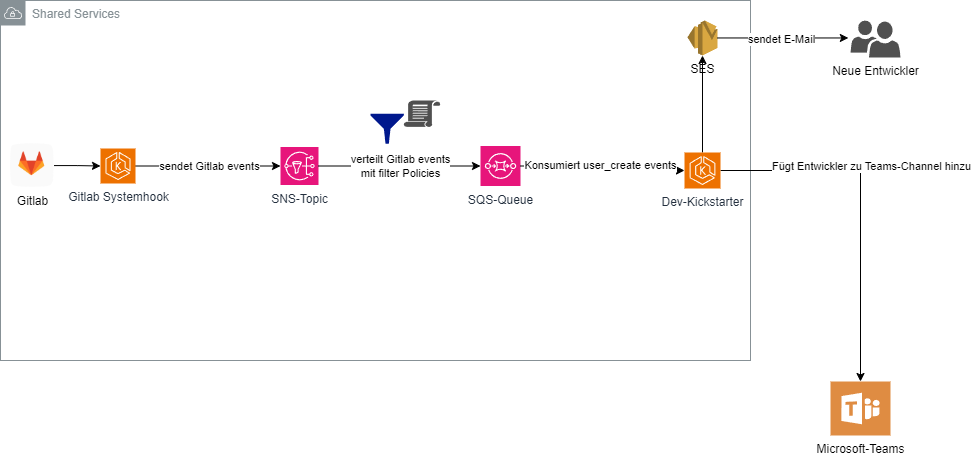
\includegraphics[scale=0.5]{final-Architektur.png}
	\caption{Finaler Entwurf des Infrastruktur-Designs und Soll-Zustand}
\end{figure}

\subsection{Architekturdesign}
\label{sec:Architekturdesign}

Für das Projekt wurde eine \textbf{ereignisgesteuerte Architektur (Event Driven Architecture)} gewählt.\footnote{Amazon Web Services - Event Driven Architecture, \cite{awsEDA}.} Diese Architektur nutzt lose gekoppelte \hyperlink{Microservices}{\textcolor{AOBlau}{Microservices}}, die Informationen durch das Erzeugen und Konsumieren von \hyperlink{GitLabEvent}{\textcolor{AOBlau}{Events}} austauschen. \hyperlink{GitLab}{\textcolor{AOBlau}{GitLab}} sendet Events über einen \hyperlink{GitLabSystemhooks}{\textcolor{AOBlau}{System Hook}} an ein \hyperlink{SNS}{\textcolor{AOBlau}{AWS SNS}}-Topic, von dem aus die Events an verschiedene \hyperlink{SQS}{\textcolor{AOBlau}{SQS Queues}} weitergeleitet werden. Diese asynchrone Kommunikation ermöglicht eine flexible und skalierbare Verarbeitung.

\subsection{Entwurf der E-Mail}
\label{sec:Benutzeroberflaeche}

Das Design der E-Mail wurde zu Beginn der Entwurfsphase skizzenhaft entworfen, um sicherzustellen, dass sie benutzerfreundlich und einladend wirkt.\footnote{Hub Spot - The Ultimate Guide to Email Design, \cite{HubSpot}.}Besonders wichtig war es, die Informationen so aufzubereiten, dass sie nicht überladen sind und die Empfänger, insbesondere neue Entwickler, schnell und einfach erfassen können. 

Die Gestaltung fokussierte sich auf eine klare und ansprechende Struktur, die dazu einlädt, die E-Mail aufmerksam zu lesen. Durch regelmäßige Rücksprache mit dem Auftraggeber und iteratives Feedback konnte das Design kontinuierlich optimiert werden. Letztlich wurde die E-Mail in \hyperlink{HTML}{\textcolor{AOBlau}{HTML}} und \hyperlink{CSS}{\textcolor{AOBlau}{CSS}} umgesetzt, um eine moderne und einladende Benutzererfahrung zu gewährleisten.

Beispielentwurf findet sich im \Anhang{app:Entwuerfe}.

\subsection{Maßnahmen zur Qualitätssicherung}
\label{sec:Qualitaetssicherung}

Um die Qualität des Projektergebnisses zu sichern, wurden verschiedene Maßnahmen ergriffen.\footnote{TU Wien - Methoden der Qualitätssicherung, \cite{Quality}}. Dazu gehören die Implementierung von \hyperlink{IntegrationTests}{\textcolor{AOBlau}{Integrationstests}} und \hyperlink{UnitTests}{\textcolor{AOBlau}{Unit-Tests}}, die automatisch bei jedem \hyperlink{GitLab}{\textcolor{AOBlau}{Git-Commit}} ausgeführt werden. Diese Tests gewährleisten, dass Änderungen am Code keine bestehenden Funktionen beeinträchtigen.

Darüber hinaus fand eine iterative Überprüfung der Codequalität durch erfahrene Mitarbeiter statt. Durch regelmäßige \hyperlink{CodeReview}{\textcolor{AOBlau}{Code-Reviews}} konnte sichergestellt werden, dass der Code den Qualitätsstandards entspricht und \hyperlink{BestPractices}{\textcolor{AOBlau}{Best Practices}} eingehalten werden. Diese Kombination aus automatisierten Tests und manuellem Feedback trägt maßgeblich zur hohen Qualität des Projekts bei.

% !TEX root = ../Projektdokumentation.tex
\section{Implementierungsphase} 
\label{sec:Implementierungsphase}

Bevor mit der Implementierung begonnen wurde, wurde ein Iterationsplan erstellt. In diesem wurden die einzelnen Schritte und deren Reihenfolge festgelegt. In jeder Iteration wurde eine spezifische Funktionalität umgesetzt und am Ende der jeweiligen Iteration dem Team präsentiert. Dieses Vorgehen folgt den in Abschnitt 2.3 beschriebenen Prinzipien der agilen Softwareentwicklung. Der vollständige Iterationsplan befindet sich im \Anhang{app:Iterationsplan}.

\subsection{Implementierung der GitLab Systemhook}
\label{sec:ImplementierungGitlabSystemhook}

Im Rahmen der Implementierung der GitLab Systemhook wurde ein Prozess entwickelt, der es ermöglicht, Ereignisse wie die Erstellung neuer Benutzer in GitLab zu erfassen und an ein SNS (Simple Notification Service) Topic weiterzuleiten. Dabei stand im Vordergrund, die Systemhook effizient, erweiterbar und in der Lage zu gestalten, Echtzeit-Benachrichtigungen für verschiedene GitLab-Ereignisse zu verarbeiten.

\begin{figure}[htb]
    \centering
    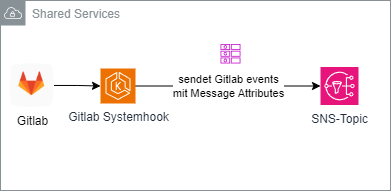
\includegraphics[scale=0.5]{systemhookOnly.drawio.png}
    \caption{Implementierung der GitLab Systemhook}
\end{figure}

Das \texttt{Hook}-Struct sowie die Initialisierung der erforderlichen Komponenten, wie dem GitLab-Client und dem AWS SNS-Client, wurden gemäß den Anforderungen definiert. Der Endpunkt, an den die HTTP-POST-Anfragen gesendet werden, ist \texttt{/api/v1/hook}. Dieser wird durch die Methode \texttt{handleHook} in der \texttt{Hook}-Struktur verarbeitet, die im Anhang~\ref{app:Test} dargestellt wird. Der Ablauf beginnt mit der Authentifizierung der HTTP-POST-Anfragen durch die Überprüfung des Tokens, um sicherzustellen, dass nur autorisierte Systeme Zugriff auf die Webhook-API erhalten. Codeauschnitte des
Authentifizierung-
sprozesses befinden sich im Anhang~\ref{app:CNMI}.

Sobald ein GitLab-Ereignis erkannt wurde, erfolgt die Verarbeitung der Payload asynchron. Durch die asynchrone Verarbeitung werden eingehende Anfragen schnell entgegengenommen und weiterverarbeitet, ohne das System zu blockieren. Im nächsten Schritt wird die empfangene Payload an den SNS-Dienst gesendet, wie in Anhang~\ref{app:CNMI} veranschaulicht. Damit die Nachrichten gezielt gefiltert und ausgewertet werden können, werden sogenannte \texttt{MessageAttributes} erstellt. Diese Attribute enthalten Informationen über das jeweilige Ereignis, wie z.B. den Ereignisnamen oder spezifische Merkmale des Benutzers, der das Ereignis ausgelöst hat. Im Falle einer Benutzererstellung wird beispielsweise geprüft, ob der neue Benutzer ein Bot ist, was ebenfalls als Attribut weitergeleitet wird.

Die \texttt{MessageAttributes} spielen eine entscheidende Rolle bei der Filterung und ermöglichen eine granulare Weiterleitung von GitLab-Ereignissen. Auf Basis dieser Attribute können spezifische Filter Policies angewendet werden, sodass nur relevante Events an nachgelagerte Systeme oder Prozesse weitergeleitet werden.



\subsection{Implementierung des Dev-Kickstarter}
\label{sec:ImplementierungBenutzeroberflaeche}

Im Rahmen der Implementierung des Dev-Kickstarter wurde eine robuste Architektur entworfen, die es ermöglicht, verschiedene Benutzerereignisse zu verarbeiten und Aktionen wie das Versenden von Willkommens-E-Mails und das Hinzufügen neuer Benutzer zu Microsoft Teams-Gruppen automatisiert auszuführen.

\begin{figure}[htb]
    \centering
    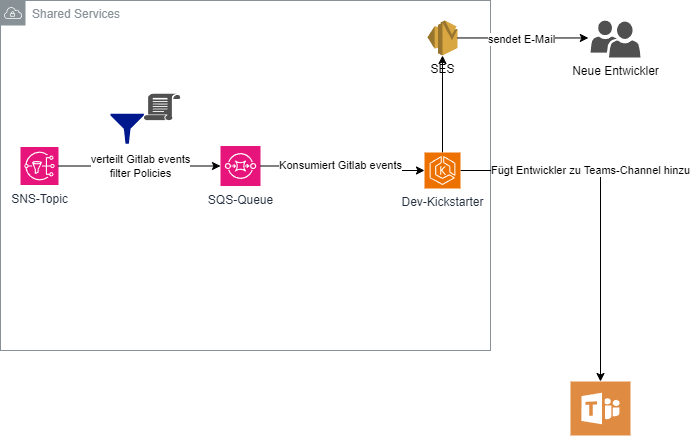
\includegraphics[scale=0.5]{dev-kickstarterOnly.drawio.png}
    \caption{Implementierung des Dev-Kickstarter}
\end{figure}

Das \texttt{Kickstarter}-Struct sowie die Initialisierung der erforderlichen Komponenten, wie dem AWS SES-Client, SQS-Consumer und Microsoft Graph-Client, wurden gemäß den Anforderungen definiert. Der SQS-Consumer empfängt Nachrichten aus einer AWS SQS-Queue, die mit Filter Policies erstellt wurde, um nur relevante Ereignisse zu verarbeiten. Die Definition der \texttt{Kickstarter}-Struktur ist im Anhang~\ref{app:kickStruct} zu finden.

Nach dem Empfang einer Nachricht wird die Payload asynchron verarbeitet. Dabei wird die E-Mail-Adresse des Benutzers extrahiert, um eine Willkommens-E-Mail über den AWS SES-Dienst zu versenden. Der zugehörige Code befindet sich im Anhang~\ref{app:kickMain}. Anschließend wird der Benutzer automatisch zu einer definierten Microsoft Teams-Gruppe hinzugefügt, indem die Microsoft Graph API verwendet wird.


\subsection{Implementierung der E-Mail}
\label{sec:ImplementierungGeschaeftslogik}

Die E-Mail wurde als HTML-Dokument erstellt, um sicherzustellen, dass sie auf verschiedenen Endgeräten und E-Mail-Clients korrekt angezeigt wird. Dabei wurde inline CSS verwendet, da viele E-Mail-Clients externe Stylesheets nicht vollständig unterstützen. Dies gewährleistet eine konsistente Darstellung der E-Mail auf allen Plattformen.

Ein wichtiges Merkmal der Implementierung ist die dynamische Personalisierung der Inhalte. Dazu wurde der Platzhalter \texttt{\{\{.FirstName\}\}} eingefügt, um den Vornamen des Empfängers einzufügen. Dieser Wert wird zur Laufzeit gefüllt, indem der Code des Empfängers ausgewertet und der entsprechende Vorname dynamisch in die Vorlage eingefügt wird.

Zusätzlich wurden nützliche Ressourcen und Links in die E-Mail integriert, wie z.B. der Zugriff auf interne TUI-Plattformen wie \textit{Runway} und \textit{OneSource}, um den neuen Teammitgliedern den Einstieg zu erleichtern. Sicherheitsaspekte wurden ebenfalls berücksichtigt, indem Links zu den TUI-Sicherheitsrichtlinien eingebunden wurden. Dies unterstreicht die Wichtigkeit des sicheren Arbeitens innerhalb der Organisation.

Wie die finale E-Mail aussieht, kann im Anhang~A.\ref{app:finalDesign} eingesehen werden.




% !TEX root = ../Projektdokumentation.tex
\section{Einführungsphase}
\label{sec:Einfuehrungsphase}

\subsection{EKS-Deployment}
\label{sec:EKSDeployment}

Die \hyperlink{GitLabSystemhooks}{\textcolor{AOBlau}{GitLab-Systemhook}} und der Dev-Kickstarter wurden im Rahmen einer automatisierten \hyperlink{CI}{\textcolor{AOBlau}{CI/CD}}-Pipeline containerisiert und anschließend in die \hyperlink{GitLab}{\textcolor{AOBlau}{GitLab-Registry}} hochgeladen. Um die Anwendungen im \hyperlink{EKS}{\textcolor{AOBlau}{Kubernetes-Cluster (EKS)}} bereitzustellen, wurde eine \hyperlink{YAML}{\textcolor{AOBlau}{yaml}}-Konfigurationsdatei erstellt. Diese Datei definiert alle notwendigen Ressourcen und Parameter, wie z.B. die \hyperlink{ContainerImage}{\textcolor{AOBlau}{Container-Images}}, \hyperlink{Ports}{\textcolor{AOBlau}{Ports}}, \hyperlink{Umgebungsvariablen}{\textcolor{AOBlau}{Umgebungsvariablen}} und \hyperlink{KubernetesIngress}{\textcolor{AOBlau}{Ingress-Konfigurationen}}.

Die fertige \hyperlink{GitCommit}{\textcolor{AOBlau}{yaml}}-Datei wurde dann in ein internes Repository commitet, welches für alle unsere EKS-Deployments verwendet wird. Sobald der \hyperlink{GitCommit}{\textcolor{AOBlau}{Commit}} erfolgt ist, wird das Deployment im Cluster automatisch ausgelöst und die Anwendungen werden dort bereitgestellt. 

Ein Beispiel für die verwendete \hyperlink{YAML}{\textcolor{AOBlau}{yaml}}-Konfiguration kann im \Anhang{app:yamlFile} eingesehen werden.

\subsection{AWS-Deployment}
\label{sec:AWSDeployment}

Für das AWS-Deployment wurden die erforderlichen Infrastrukturkomponenten in der AWS-Umgebung konfiguriert. Dazu gehören \hyperlink{SNS}{\textcolor{AOBlau}{Amazon SNS}} zur Kommunikation und \hyperlink{SQS}{\textcolor{AOBlau}{Amazon SQS}} zur Nachrichtenverarbeitung. 

Die Bereitstellung dieser Ressourcen erfolgte mithilfe von \hyperlink{InfrastructureAsCode}{\textcolor{AOBlau}{Infrastructure as Code}} mit \hyperlink{Terraform}{\textcolor{AOBlau}{Terraform}}.\footnote{Spacelift - Infrastructure as Code, \cite{Iac}.} Dabei wurden \hyperlink{SNS}{\textcolor{AOBlau}{SNS-Topics}} und \hyperlink{SQS}{\textcolor{AOBlau}{SQS-Queues}} eingerichtet, um die Kommunikation zwischen den Diensten zu ermöglichen. Eine \hyperlink{FilterPolicies}{\textcolor{AOBlau}{Filter-Policy}} wurde verwendet, um sicherzustellen, dass nur spezifische Ereignisse, wie das Erstellen eines Benutzers (eventName: \texttt{user\_create}), an die \hyperlink{SQS}{\textcolor{AOBlau}{SQS-Queue}} weitergeleitet werden. 

Zusätzlich wurde eine \hyperlink{SES}{\textcolor{AOBlau}{IAM-Policy}} erstellt, die dem Dev-Kickstarter die erforderlichen Berechtigungen gewährt, um E-Mails über \hyperlink{SES}{\textcolor{AOBlau}{Amazon SES}} zu senden und Nachrichten aus der \hyperlink{SQS}{\textcolor{AOBlau}{SQS-Queue}} zu empfangen. 

Die \hyperlink{Terraform}{\textcolor{AOBlau}{Terraform}}-Ressourcen sind in einem internen Repository gespeichert. Ein Beispiel für die verwendeten \hyperlink{Terraform}{\textcolor{AOBlau}{Terraform}}-Ressourcen kann im \Anhang{app:terraform} eingesehen werden.

% !TEX root = ../Projektdokumentation.tex
\section{Abnahmephase} 
\label{sec:Abnahmephase}

Vor der Endabnahme wurden umfangreiche Tests durchgeführt, um die Qualität der Anwendung sicherzustellen. Unit-Tests prüften die Funktionalität einzelner Codebestandteile isoliert, deren Logs im \Anhang{app:Test} zu finden sind. Integrationstests überprüften, ob die einzelnen Module korrekt zusammenarbeiten und die definierten Schnittstellen erfolgreich miteinander kommunizieren.

Nachdem die Anwendung fertiggestellt war, konnte sie zur Endabnahme dem Fachbereich vorgelegt werden. Durch die agile Entwicklungsmethode hatte der Fachbereich nach jeder Iteration Zugriff auf aktuelle Versionen der Anwendung und konnten so frühzeitig Feedback geben. Diese regelmäßigen Rücksprachen führten nicht nur zu einer vertrauten Nutzung, sondern auch zu einem tiefen Verständnis der Funktionsweise des Gesamtsystems. Anregungen und Kritik konnten direkt während der Entwickl-
ung berücksichtigt werden, wodurch bereits viele Probleme frühzeitig behoben werden konnten.

Da die Fachbereiche die Anwendung bereits gut kannten, verlief die Endabnahme reibungslos. Zur zusätzlichen Qualitätssicherung wurde vor dem Deployment ein \hyperlink{CodeReview}{\textcolor{AOBlau}{Code Review}} durch einen weiteren Entwickler durchgeführt, und die Einführung der Anwendung konnte erfolgreich abgeschlossen werden.

% !TEX root = ../Projektdokumentation.tex
\section{Dokumentation}
\label{sec:Dokumentation}

Die \textbf{Projektdokumentation} beschreibt den gesamten Verlauf der Projektumsetzung, einschließlich der Planung, Durchführung und Tests. Sie dient als Referenz für alle Projektbeteiligten und dokumenti-
ert die wichtigsten Phasen und Entscheidungen im Projekt. IT-spezifische Fachbegriffe werden dabei, soweit möglich, vermieden, um die Verständlichkeit für alle Beteiligten zu gewährleisten.

Die \textbf{Entwicklerdokumentation} enthält die technischen Anforderungen, Konfigurationsparameter und Endpunkte der Anwendung. Sie bietet detaillierte Informationen zu \hyperlink{Umgebungsvariablen}{\textcolor{AOBlau}{Umgebungsvariablen}}, \hyperlink{Flags}{\textcolor{AOBlau}{Flags}} und \hyperlink{Endpoints}{\textcolor{AOBlau}{Endpunkte}} für die Einrichtung und das Deployment der Anwendung. Ein Auszug dieser Dokumen-
tation ist im \Anhang{app:Doc} zu finden.

Die Dokumentationen sind so formuliert, dass sie den Anforderungen der jeweiligen Verwendung gerecht werden. Die Projektdokumentation ist allgemein verständlich formuliert, während die Entwickl-
erdokumentation technische Details und Anweisungen für die Konfiguration und den Betrieb der Anwendung enthält.

\section{Fazit} 
\label{sec:Fazit}

\subsection{Soll-/Ist-Vergleich}
\label{sec:SollIstVergleich}

Bei einer rückblickenden Betrachtung des Projekts lässt sich festhalten, dass die festgelegten Anforderungen weitgehend erreicht wurden. Alle wesentlichen Funktionen und Anpassungen wurden gemäß den definierten Zielen und Anforderungen umgesetzt.

Die Projektplanung konnte insgesamt eingehalten werden, obwohl kleinere Abweichungen in einzelnen Phasen auftraten. So war in der Dokumentationsphase ein Mehraufwand erforderlich, während die Test- und Kontrollphase weniger Zeit in Anspruch nahm. Diese Abweichungen konnten innerhalb des geplanten Zeitrahmens ausgeglichen werden, sodass das Projekt planmäßig abgeschlossen werden konnte. Die folgende Tabelle zeigt den Soll-/Ist-Vergleich der Projektphasen:

\begin{table}[h]
\centering
\caption{Soll-/Ist-Vergleich}
\label{tab:Vergleich}
\begin{tabular}{|l|c|c|c|}
\hline
\textbf{Projektphase} & \textbf{Geplante Zeit} & \textbf{Tatsächliche Zeit} & \textbf{Differenz} \\
\hline
Analysephase & 6 h & 6 h & 0 h \\
\hline
Entwurfsphase & 6 h & 6 h & 0 h \\
\hline
Implementierungsphase & 34 h & 34 h & 0 h \\
\hline
Test- und Kontrollphase & 18 h & 16 h & -2 h \\
\hline
Dokumentation + Nachbearbeitung & 6 h & 8 h & +2 h \\
\hline
Erstellen der Projektdokumentation und Präsentation & 8 h & 10 h & +2 h \\
\hline
Pufferzeit & 2 h & 0 h & -2 h \\
\hline
\textbf{Gesamt} & \textbf{80 h} & \textbf{80 h} & \textbf{0 h} \\
\hline
\end{tabular}
\end{table}

Der Auftraggeber zeigte sich mit dem Projektergebnis zufrieden, da alle zentralen Anforderungen erfüllt und interne Abläufe optimiert wurden.

\subsection{Lessons Learned}
\label{sec:LessonsLearned}

Im Verlauf des Projekts konnten wertvolle Erfahrungen gesammelt werden, insbesondere hinsichtlich der effizienten Planung und Einhaltung von Projektphasen in einem agilen Umfeld. Die kontinuierliche Rücksprache mit dem Fachbereich erwies sich als entscheidend für die erfolgreiche Umsetzung der Projektanforderungen. Auch die Anwendung der \hyperlink{agil}{\textcolor{AOBlau}{agilen}} Entwicklungsweise und die regelmäßige Einbeziehung der Endnutzer sorgten für eine zielgerichtete und bedarfsorientierte Entwicklung.

\subsection{Ausblick}
\label{sec:Ausblick}

Obwohl alle definierten Anforderungen im Projekt umgesetzt wurden, gibt es Potenzial für zukünftige Erweiterungen. Eine mögliche Weiterentwicklung wäre die Ergänzung zusätzlicher Schnittstellen, um eine automatisierte Anbindung weiterer interner Systeme zu ermöglichen. Auch die Weiterentwicklung der bestehenden Funktionen für eine noch tiefere Integration in die vorhandene Infrastruktur wäre sinnvoll.

Aufgrund des modularen Aufbaus der Anwendung, wie im Abschnitt \ref{sec:Architekturdesign} beschrieben, können diese Anpassungen und Erweiterungen problemlos vorgenommen werden. Der flexible Aufbau der Anwendung gewährleistet somit eine gute Wartbarkeit und Erweiterbarkeit für zukünftige Anforderungen.


% Literatur ------------------------------------------------------------------
\clearpage
\renewcommand{\refname}{Literaturverzeichnis}
\bibliography{Bibliographie}
\bibliographystyle{Allgemein/natdin} % DIN-Stil des Literaturverzeichnisses
\input{Erklaerung}

% Anhang ---------------------------------------------------------------------
\clearpage
\appendix
\pagenumbering{roman}
% !TEX root = Projektdokumentation.tex
\section{Anhang}
\subsection{Detaillierte Zeitplanung}
\label{app:Zeitplanung}

\tabelleAnhang{ZeitplanungKomplett}
\clearpage
\subsection{Ressourcen Planung}
\label{app:Ressourcen}
\textbf{Hardware}
\begin{itemize}
    \item Büroarbeitsplatz mit Thin-Client
\end{itemize}

\textbf{Software}
\begin{itemize}
    \item Windows 7 Enterprise mit Service Pack 1 - Betriebssystem
    \item Visual Studio Code - Hauptentwicklungsumgebung
    \item Docker - Containerisierung von Anwendungen
    \item Go - Programmiersprache zur Entwicklung des Webservers
    \item AWS - Cloud-Infrastruktur
    \item EKS (Elastic Kubernetes Service) - Orchestrierung der Container
    \item Terraform - Infrastruktur als Code
    \item GitLab - Versionskontrolle und CI/CD
    \item MS Teams - Zusammenarbeit im Team
    \item Jira - Projektmanagement
\end{itemize}

\textbf{Personal}
\begin{itemize}
    \item Entwickler - Umsetzung des Projektes
    \item Anwendungsentwickler - Review des Codes
\end{itemize}


\input{Anhang/AnhangLastenheft.tex}
\clearpage

\subsection{Use Case-Diagramm}
\label{app:UseCase}
Use Case-Diagramme und weitere \acs{UML}-Diagramme kann man auch direkt mit \LaTeX{} zeichnen, siehe \zB \url{http://metauml.sourceforge.net/old/usecase-diagram.html}.
\begin{figure}[htb]
\centering
\includegraphicsKeepAspectRatio{UseCase.pdf}{0.7}
\caption{Use Case-Diagramm}
\end{figure}

\input{Anhang/AnhangPflichtenheft.tex}

\subsection{Datenbankmodell}
\label{app:Datenbankmodell}
ER-Modelle kann man auch direkt mit \LaTeX{} zeichnen, siehe \zB \url{http://www.texample.net/tikz/examples/entity-relationship-diagram/}.
\begin{figure}[htb]
\centering
\includegraphicsKeepAspectRatio{database.pdf}{1}
\caption{Datenbankmodell}
\end{figure}
\clearpage

\subsection{Oberflächenentwürfe}
\label{app:Entwuerfe}
\begin{figure}[htb]
\centering
\includegraphicsKeepAspectRatio{mailSkizze.png}{0.7}
\caption{Erster Entwurf der E-Mail}
\end{figure}

\begin{figure}[htb]
\centering
\includegraphicsKeepAspectRatio{firstMail.png}{0.7}
\caption{Umsetzung in HTML mit CSS}
\end{figure}

\begin{figure}[htb]
\centering
\includegraphicsKeepAspectRatio{finalMail.png}{0.7}
\caption{Finales Design der E-Mail}
\end{figure}

\clearpage
\subsection{Screenshot der versendeten E-Mail}
\label{Screenshots}
\begin{figure}[htb]
    \centering
    \includegraphicsKeepAspectRatio{finalMail.png}{0.7}
    \caption{Finales Design der E-Mail}
    \label{app:finalDesign}
    \end{figure}


\subsection{Entwicklerdokumentation (Auszug)}
\label{app:Doc}
\begin{figure}[htb]
\centering
\includegraphicsKeepAspectRatio{enwicklerdoc.png}{1.1}
\caption{Entwicklerdokumentation}
\end{figure}

    
\clearpage
\subsection{Initialisierung der Hook-Struktur}
\label{app:Test}
\lstinputlisting[language=go, caption={Initialisierung der Hook-Struktur}]{Listings/hookStruktur.go}
\clearpage


\subsection{Klasse: ComparedNaturalModuleInformation}
\label{app:CNMI}
Kommentare und simple Getter/Setter werden nicht angezeigt.
\lstinputlisting[language=php, caption={Klasse: ComparedNaturalModuleInformation}]{Listings/cnmi.php}
\clearpage

\subsection{Klassendiagramm}
\label{app:Klassendiagramm}
Klassendiagramme und weitere \acs{UML}-Diagramme kann man auch direkt mit \LaTeX{} zeichnen, siehe \zB \url{http://metauml.sourceforge.net/old/class-diagram.html}.
\begin{figure}[htb]
\centering
\includegraphicsKeepAspectRatio{Klassendiagramm.pdf}{1}
\caption{Klassendiagramm}
\end{figure}
\clearpage

\input{Anhang/AnhangBenutzerDoku.tex}


\end{document}
